Un conversor digital--analógico (CDA) es un circuito electrónico que transforma una
señal digital, generalmente un número binario, en una señal analógica continua,
p.ej, un voltaje. Es especialmente útil en dispositivos como altavoces, dado que
convierte el flujo de datos en formato digital a señales de audio analógicas.

El principio de funcionamiento del CDA consiste en la división de voltaje controlada
por los bits de entrada de la señal digital. El ejemplo más simple para un CDA es
un generador de voltaje proporcional a un número binario $Q$ dado por
\begin{equation}\label{eq:Q}
	Q = \sum_{i=0}^{n-1} 2^ib_i,
\end{equation}
donde $b_i$ son los i-ésimos digitos de un número binario con $n$ digitos totales.
El circuito de la Fig. \ref{fig:circuito} representa el generador de voltaje mencionado
con tres bits de entrada.
\begin{figure}[H]
	\centering
	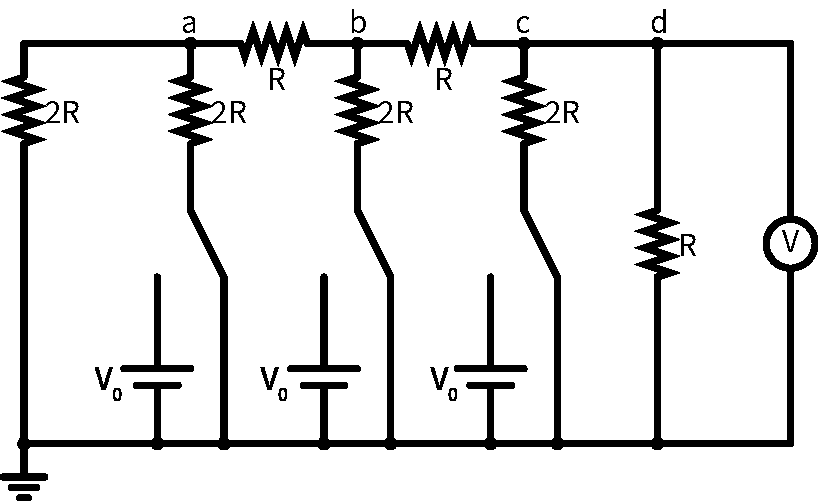
\includegraphics[width=0.9\linewidth]{res/circuitoAsset-1.pdf}
	\caption{Circuito CDA; generador de voltaje analógico proporcional a una
	señal digital binaria. $R$ corresponde a una resistencia arbitraria
	y $V_0$ al voltaje a dividir. Cada interruptor actúa como un bit del número
	binario de derecha a izquierda.}
	\label{fig:circuito}
\end{figure}
Con esto, para determinar el voltaje $V_{\text{out}}$ leído por el voltímetro
para cualquier combinación de bits, es necesario utilizar el principio de superposición.
Suponiendo que $V_i$ es el voltaje leído cuando el i-ésimo bit es 1, mientras el resto es
0, $V_{\text{out}}$ se puede escribir como
\begin{equation}\label{eq:out}
	V_{\text{out}} = \sum_{i=0}^{n-1}V_i b_i.
\end{equation}
Asi, solo queda determinar los voltajes $V_i$ utilizando el teorema de Thévenin entre
los nodos $(a,\Ground{})$, $(b,\Ground{})$, $(c,\Ground{})$ y $(d,\Ground{})$.
Para cada uno de los casos anteriores, el circuito equivalente de Thevenin entre un
nodo $k$ y $\Ground{}$ puede tomar una de dos formas: la Fig. \ref{fig:T1},
\textit{antes} del bit encendido, y la Fig. \ref{fig:T2}, \textit{en} y \textit{después}
del bit encendido. El circuito equivalente en ambas figuras divide a la mitad las
resistencias en paralelo y el voltaje.
\begin{figure}[H]
	\centering
	\begin{subfigure}[H]{0.9\linewidth}
		\centering
		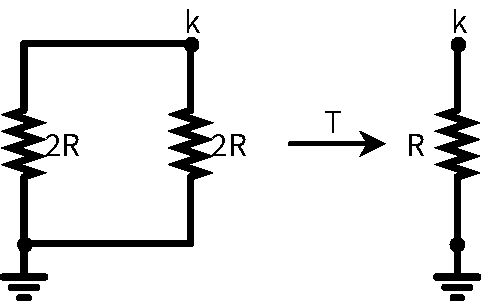
\includegraphics[width=0.8\linewidth]{res/T1Asset-1.pdf}
		\caption{Comparación entre una sección del circuito \ref{fig:circuito} antes del
		bit encendido y su equivalente.}
		\label{fig:T1}
	\end{subfigure}
	%
	\begin{subfigure}[H]{0.9\linewidth}
		\centering
		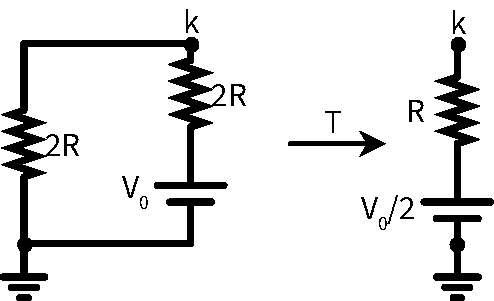
\includegraphics[width=0.8\linewidth]{res/T2Asset-2.pdf}
		\caption{Comparación entre una sección del circuito \ref{fig:circuito} en y
		después del bit encendido y su equivalente.}
		\label{fig:T2}
	\end{subfigure}
	\caption{Configuraciones posibles entre un nodo $k$ del circuito
	\ref{fig:circuito} y sus equivalentes de Thevenin.}
\end{figure}
Realizando este procedimiento para cada una de las configuraciones de bits, se tiene
que
\begin{align*}
	V_1 &= \frac{V_0}{16} \\
	V_2 &= \frac{V_0}{8} \\
	V_3 &= \frac{V_0}{4},
\end{align*}
por lo que $V_{\text{out}}$ para $n=3$ queda como
\begin{equation}\label{eq:out}
	V_{\text{out}} = V_0\left( \frac{b_1}{16} + \frac{b_2}{8} + \frac{b_3}{4}\right)
\end{equation}
En ese sentido, en el presente informe se analizó el voltaje generado por un CDA
con el fin de comprobar la relación deducida por el teorema de Thevenin. Comprobar
la relación implica replicar los posibles valores teóricos para tres bits; es decir,
los números del 0 al 7 en voltios para un valor de $V_0=\qty{16}{\volt}$, dentro de un
margen de error adecuado.